%
% $LastChangedRevision: 1896 $
% $LastChangedDate:: 2020-04-29 15:30:11 +0200#$
%
% This file is part of X2C. http://x2c.lcm.at/
%
% Copyright (c) 2019, Linz Center of Mechatronics GmbH (LCM) http://www.lcm.at/
% All rights reserved.
%
%
% This file is licensed according to the BSD 3-clause license as follows:
%
% Redistribution and use in source and binary forms, with or without
% modification, are permitted provided that the following conditions are met:
%     * Redistributions of source code must retain the above copyright
%       notice, this list of conditions and the following disclaimer.
%     * Redistributions in binary form must reproduce the above copyright
%       notice, this list of conditions and the following disclaimer in the
%       documentation and/or other materials provided with the distribution.
%     * Neither the name of the "Linz Center of Mechatronics GmbH" and "LCM" nor
%       the names of its contributors may be used to endorse or promote products
%       derived from this software without specific prior written permission.
%
% THIS SOFTWARE IS PROVIDED BY THE COPYRIGHT HOLDERS AND CONTRIBUTORS "AS IS" AND
% ANY EXPRESS OR IMPLIED WARRANTIES, INCLUDING, BUT NOT LIMITED TO, THE IMPLIED
% WARRANTIES OF MERCHANTABILITY AND FITNESS FOR A PARTICULAR PURPOSE ARE DISCLAIMED.
% IN NO EVENT SHALL "Linz Center of Mechatronics GmbH" BE LIABLE FOR ANY
% DIRECT, INDIRECT, INCIDENTAL, SPECIAL, EXEMPLARY, OR CONSEQUENTIAL DAMAGES
% (INCLUDING, BUT NOT LIMITED TO, PROCUREMENT OF SUBSTITUTE GOODS OR SERVICES;
% LOSS OF USE, DATA, OR PROFITS; OR BUSINESS INTERRUPTION) HOWEVER CAUSED AND
% ON ANY THEORY OF LIABILITY, WHETHER IN CONTRACT, STRICT LIABILITY, OR TORT
% (INCLUDING NEGLIGENCE OR OTHERWISE) ARISING IN ANY WAY OUT OF THE USE OF THIS
% SOFTWARE, EVEN IF ADVISED OF THE POSSIBILITY OF SUCH DAMAGE.
%
\ifdefined\Matlab

\XtoCBlock{Start Simulation (Simulink only)}
\label{block:StartSimulation}
\begin{figure}[H]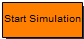
\includegraphics{Icons/StartSimulation}\end{figure} 

\subsubsection*{Description:}
With a double-click on this block, the Simulink model will be analyzed (to enter the correct sample time values in each of the blocks) and the solver will be set to \textit{FixedStepDiscrete} with its step size set to the model sample time. Then the simulation will be started.

\fi